\documentclass[a4paper,12pt, french]{report}

\usepackage{fancyhdr}

% Utilisation de tous les packages nécéssaires

\usepackage[utf8]{inputenc}
\usepackage[utf8]{inputenc}%           gestion des accents (source)
\usepackage[T1]{fontenc}%              gestion des accents (PDF)
\usepackage[francais]{babel}%          gestion du français
\usepackage{textcomp}%                 caractères additionnels
\usepackage{lmodern}%                  police de caractère
\usepackage{geometry}%                 gestion des marges
\usepackage{graphicx}%                 gestion des images
\usepackage{array}%                    gestion améliorée des tableaux
\usepackage{calc}%                     syntaxe naturelle pour les calculs
\usepackage{amsmath}
\usepackage{dsfont}
\usepackage{color}
\usepackage{url}
\usepackage{hyperref}
\usepackage{listings} %Algorithmes
\usepackage{listingsutf8}
\usepackage{xcolor}
\usepackage{caption}
\DeclareCaptionFont{white}{\color{white}}



\definecolor{mygreen}{rgb}{0,0.6,0}
\definecolor{mygray}{rgb}{0.5,0.5,0.5}
\definecolor{mymauve}{rgb}{0.58,0,0.82}

\graphicspath{ {images/} }


\hypersetup{
colorlinks=true, %colorise les liens
breaklinks=true, %permet le retour à la ligne dans les liens trop longs
urlcolor= blue, %couleur des hyperliens
linkcolor= black, %couleur des liens internes
citecolor=blue,    %couleur des liens de citations
}


\definecolor{Comments}{rgb}{0.13,0.54,0.13}
\definecolor{Strings}{rgb}{0,0.63,0}
\definecolor{Keywords}{rgb}{0,0,1}
\definecolor{Background}{rgb}{1,1,1}
\definecolor{Variables}{rgb}{0.62, 0.12, 0.94}

\tolerance=1000

\title{PAO: Développement d'une bibliothèque musicale}
\author{Alexis \bsc{Durieux}}
\date{ASI4 - 2017}

\pagestyle{fancy}
\fancyhead[R]{}
\fancyhead[L]{
\includegraphics[scale=0.35]{insa-logo.png}}

\begin{document}
\maketitle
\tableofcontents

\chapter*{Introduction}
L'objectif de ce PAO est la mise en application des concepts de bases de données par la mise en place d'une base de données et de son utilisation pour réaliser un ensemble de fonctionnalités. Dans notre cas, l'objectif est la création d'une bibliothèque musicale permettant à un utilisateur l'enregistrement de sa discographie. Pour concevoir cette base de données au mieux nous allons procéder par étapes. Dans un premier temps, nous allons analyser les besoins de l'application, puis nous allons réaliser le modèle entité-attribut avant de passer au modèle relationnel. Avec la base de données créée nous allons pouvoir réaliser une application java simple basée sur cette dernière. Nous implémenterons ensuite le pattern \textbf{DAO} afin de passer du \emph{modèle relationnel} à un \emph{modèle objet}. En terme de technologie, nous utiliserons une base de données \emph{Postgres} et \emph{JDBC} pour faire le liant avec l'application JAVA afin d'implémenter le pattern \textbf{DAO}

\chapter{Analyse des besoins de l'application}
Nous voulons donc créer une application permettant à l'utilisateur d'enregistrer ses musiques, artistes et albums afin de pouvoir les consulter. L'utilisateur utilise la bibliothèque de l'application pour ajouter ces derniers à sa  bibliothèque personnelle. Néanmoins l'utilisateur peut ajouter directement des musiques, albums et artistes à sa bibliothèque personnelle qui sont donc ajoutés à la bibliothèque de l'application. C'est donc une bibliothèque musicale collaborative que nous cherchons à créer où les données ajoutées par un utilisateur servent à tous les utilisateurs. On suppose également les relations suivantes. Un titre est contenu dans un album et un album est composé par un artiste. Ces relations sont primordiales à la bonne création de nos tables. En plus de vouloir stocker des titres, artistes et albums, on veut également stocker des informations propres à l'utilisateur. Enfin ce dernier doit être en mesure de stocker des écoutes et de créer et modifier des playlists. On suppose enfin qu'une fois créé un titre ne peut être modifié ou supprimé de la bibliothèque de l'application. En effet une modification par un utilisateur engendrera sinon une modification potentielle dans la bibliothèque d'autres utilisateurs.
\chapter{Modèle entité-attribut et relationnel}
\section{Modélisation entité-attribut}
  \includegraphics[scale=0.5]{ea-final.png}
\section{Modélisation de la vue}
  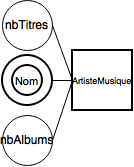
\includegraphics[scale=0.7]{vues.png}
\section{Du modèle entité-attribut vers le modèle relationnel}
  \subsection{Tables, clés primaires et cardinalité}
    \begin{itemize}
      \item Utilisateur(\underline{pseudo}, motDePasse, nom, prenom, age) \newline
        La table \emph{Utilisateur} référence les utilisateurs. On choisit comme \textbf{clé primaire} un \emph{pseudo} en raison des homonymes possibles entre utilisateurs.
      \item Titre(\underline{id}, nom, duree, nomAlbum, genre) \newline
        La table \emph{Titre} référence les titres. On choisit un \textbf{id} \textbf{clé primaire} en raison des homonymies possibles entre \textbf{plusieurs} titres. On a également un \emph{nomAlbum} afin de représenter la cardinalité. En effet on suppose qu'un titre n'appartient au plus qu'à un seul album. Le \emph{genre} quand à lui est un attribut issu d'une énumération définissant une liste de genre de musique.
       \item Album(\underline{nom}, nomArtiste, annee) \newline
        La table \emph{Album} référence les albums. On suppose dans notre cas que deux albums ne peuvent avoir le même nom. On peut donc choisir \textbf{nom} comme \textbf{clé primaire}. La clé étrangère \emph{nomArtiste} représente le fait qu'un album est composé par un seul artiste.
      \item Artiste(\underline{nom}, nationalite) \newline
        La table \emph{Artiste} référence les \emph{artistes}. Ici on a choisit comme \textbf{clé primaire} le \emph{nom} car on suppose que deux artistes ne peuvent pas avoir le même nom.
      \item ListeTitre(\underline{pseudoUser}, \underline{titreId}) \newline
        La table \emph{ListeTitre} correspond aux titres enregistrés par un utilisateur dans sa bibliothèque. On associe un utilisateur à un titre. La \textbf{clé primaire}: est \textbf{(pseudoUser, titreId)} car un utilisateur ne peut enregistrer deux titres identiques dans sa bibliothèque. En revanche un titre peut être enregistré dans la bibliothèque respective de \textbf{plusieurs} utilisateurs.
      \item ListeAlbum(\underline{pseudoUser}, \underline{nomAlbum}) \newline
        La table \emph{ListeAlbum} correspond aux albums enregistrés par un utilisateur dans sa bibliothèque. On associe un utilisateur à un titre. La \textbf{clé primaire}: est \textbf{(pseudoUser, nomAlbum)} car un utilisateur ne peut enregistrer deux albums identiques dans sa bibliothèque. En revanche un album peut être enregistré dans la bibliothèque respective de \textbf{plusieurs} utilisateurs.
      \item ListeArtiste(\underline{pseudoUser}, \underline{nomArtiste}) \newline
        La table \emph{ListeArtiste} correspond aux artistes enregistrés par un utilisateur dans sa bibliothèque. On associe un \textbf{utilisateur} à un \textbf{artiste}. La \textbf{clé primaire}: est \textbf{(pseudoUser, nomArtiste)} car un utilisateur ne peut enregistrer deux artistes identiques dans sa bibliothèque. En revanche un artiste peut être enregistré dans la bibliothèque respective de \textbf{plusieurs} utilisateurs.
      \item Ecoute(\underline{pseudoUser}, \underline{date}, idTitre) \newline
        La table \emph{Ecoute} correspond à une liste d'écoute. À un instant \emph{t}, un utilisateur écoute un titre. On les associe donc dans la table. On choisit comme \textbf{clé primaire}: \textbf{(pseudoUser, date)}. En effet, un utilisateur ne peut écouter deux musiques en même temps.
      \item Playlist(\underline{id}, pseudoUser, nom) \newline
        La table \emph{Playlist} référence les playlists des utilisateurs. La \textbf{clé primaire} est un \emph{id} car un utilisateur peut avoir \textbf{plusieurs} playlists. On ne peut également choisir le \emph{nom} car deux utilisateurs différents peuvent avoir une playlist ayant le même nom. En raison de la table \textbf{PlaylistTitre}, on utilise \textbf{id} comme clé primaire car clé étrangère de \textbf{PlaylistTitre}.
      \item PlaylistTitre(\underline{idTitre}, \underline{idPlaylist}) \newline
        La table \emph{PlaylistTitre} référence les titres des playlists. La \textbf{clé primaire} est \textbf{(idTitre, idPlaylist)} car un titre peut être présent une seule fois dans une même \emph{playlist} mais être présent dans \textbf{plusieurs} playlists différentes.
    \end{itemize}
  \subsection{Vue}
    \begin{itemize}
       \item  La \textbf{vue} \emph{ArtisteMusique} agrège un \emph{artiste} avec son \emph{nombre de titres} et \emph{nombre d'albums} calculés respectivement à partir des tables \emph{Titre} et \emph{Artiste}.
       Pour créer cette vue, on effectue deux jointures successives. Une première entre les tables \textbf{Artiste} et \textbf{Album} puis entre le résultat et la table \textbf{Titre}. Enfin on groupe les résultats par \emph{artistes} et on il reste à compter.
       \begin{lstlisting}[language=SQL, label=creation-vue,caption=Création de la vue , breaklines, frame=single]{vue.sql}
       CREATE VIEW ArtisteVue AS SELECT nomArtiste, COUNT(DISTINCT(nomAlbum)) AS nbAlbums, COUNT(DISTINCT(nomTitre)) AS nbTitres FROM (SELECT art.nom AS nomArtiste, alb.nom AS nomAlbum, tit.nom AS nomTitre FROM ARTISTE art INNER JOIN ALBUM alb ON alb.nomartiste = art.nom INNER JOIN TITRE tit on tit.nomAlbum=alb.nom) v group by v.nomArtiste;
       \end{lstlisting}
       
    \end{itemize}

\section{Contraintes d'intégrité et types}
  \subsection{Définitions des types et tables}
    \begin{itemize}
      \item \underline{GENRE\_MUSIQUE - ÉNUMÉRATION}
        \begin{itemize}
          \item \textbf{pop, rock, jazz, blues, electronique, variété, rap, reggae}
        \end{itemize}
      \item \underline{Utilisateur}
        \begin{itemize}
          \item pseudo: \textbf{VARCHAR(15) PRIMARY KEY}
          \item motDePasse: \textbf{VARCHAR(64) NOT NULL}
          \item nom: \textbf{VARCHAR(15)}
          \item prenom: \textbf{VARCHAR(15)}
          \item age: \textbf{INTEGER} $\in ]0, 99[$
        \end{itemize}
      \item Titre
        \begin{itemize}
          \item id: \textbf{INTEGER PRIMARY KEY}
          \item nom: \textbf{VARCHAR(50) NOT NULL}
          \item duree: \textbf{INTEGER NOT NULL}
          \item nomArtiste: \textbf{VARCHAR(25) FOREIGN KEY REFERENCES ARTISTE NOT NULL}
          \item nomAlbum: \textbf{VARCHAR(25) FOREIGN KEY REFERENCES ALBUM}
          \item genre: \textbf{GENRE\_MUSIQUE}
r la valeur de \textbf{id}
        \end{itemize}
      \item Album
        \begin{itemize}
          \item nom: \textbf{VARCHAR(25) PRIMARY KEY}
          \item nomArtiste: \textbf{VARCHAR(25) REFERENCES ARTISTE NOT NULL}
          \item annee: \textbf{INTEGER} $\in ]0, 3000[$
        \end{itemize}
      \item Artiste
        \begin{itemize}
          \item nom: \textbf{VARCHAR(25) PRIMARY KEY}
          \item nationalite: \textbf{VARCHAR(50)}
        \end{itemize}
      \item ListeTitre
        \begin{itemize}
          \item pseudoUser: \textbf{VARCHAR(15) FOREIGN KEY REFERENCES UTILISATEUR}
          \item titreId: \textbf{INTEGER FOREIGN KEY REFERENCES TITRE}
          \item \textbf{PRIMARY KEY: (pseudoUser, titreId)}
        \end{itemize}
      \item ListeAlbum
        \begin{itemize}
          \item pseudoUser: \textbf{VARCHAR(15) FOREIGN KEY REFERENCES UTILISATEUR}
          \item nomAlbum: \textbf{VARCHAR(25) FOREIGN KEY REFERENCES ALBUM}
          \item \textbf{PRIMARY KEY: (pseudoUser, nomAlbum)}
        \end{itemize}
      \item ListeArtiste
        \begin{itemize}
          \item pseudoUser: \textbf{VARCHAR(15) FOREIGN KEY REFERENCES UTILISATEUR}
          \item nomArtiste: \textbf{VARCHAR(25) FOREIGN KEY REFERENCES ARTISTE}
          \item \textbf{PRIMARY KEY: (pseudoUser, nomArtiste)}
        \end{itemize}
      \item Ecoute
        \begin{itemize}
          \item pseudoUser: \textbf{VARCHAR(15) FOREIGN KEY REFERENCES UTILISATEUR}
          \item dateEcoute: \textbf{TIMESTAMP DEFAULT CURRENT\_TIMESTAMP}
          \item titreId: \textbf{INTEGER FOREIGN KEY REFERENCES TITRE}
          \item \textbf{PRIMARY KEY: (pseudoUser, dateEcoute)}
        \end{itemize}
      \item Playlist
        \begin{itemize}
          \item id: \textbf{VARCHAR(10) PRIMARY KEY}
          \item nom: \textbf{VARCHAR(25) NOT NULL}
          \item pseudoUser: \textbf{VARCHAR(15) FOREIGN KEY REFERENCES UTILISATEUR}
          Il faut noter qu'on utilise une \textbf{séquence} de \textbf{INTEGER} pour définir la valeur de \textbf{id}
        \end{itemize}
      \item PlaylistTitre
        \begin{itemize}
          \item titreId: \textbf{INTEGER FOREIGN KEY REFERENCES TITRE}
          \item playlistId: \textbf{INTEGER FOREIGN KEY REFERENCES PLAYLIST}
          \item \textbf{PRIMARY KEY: (titreId, playlistId)}
        \end{itemize}
      \end{itemize}
	  \begin{lstlisting}[language=SQL, label=creation-tables,caption=Création des tables, breaklines, frame=single]
	  CREATE TYPE GENRE_MUSIQUE AS ENUM(
	  'pop', 'rock', 'jazz', 'blues', 'electronique', 'variete', 'rap', 'reggae'
	  );
	  
	  CREATE SEQUENCE TITRE_SEQ
	  start 1
	  increment 1
	  NO MAXVALUE
	  CACHE 1;
	  
	  CREATE SEQUENCE PLAYLIST_SEQ
	  start 1
	  increment 1
	  NO MAXVALUE
	  CACHE 1;
	  
	  CREATE TABLE UTILISATEUR(
	  pseudo VARCHAR(15) PRIMARY KEY,
	  motDePasse VARCHAR(64) NOT NULL,
	  nom VARCHAR(15),
	  prenom VARCHAR(15),
	  age INTEGER CONSTRAINT age_constraint CHECK (age > 0 AND age < 99)
	  );
	  
	  CREATE TABLE ARTISTE(
	  nom VARCHAR(25) PRIMARY KEY,
	  nationalite VARCHAR(50)
	  );
	  
	  CREATE TABLE ALBUM(
	  nom VARCHAR(25) PRIMARY KEY,
	  nomArtiste VARCHAR(25) REFERENCES ARTISTE NOT NULL,
	  annee INTEGER CONSTRAINT year_constraint CHECK (annee > 0 AND annee < 3000)
	  );
	  
	  CREATE TABLE TITRE( 
	  id INTEGER PRIMARY KEY DEFAULT nextval('TITRE_SEQ'),
	  nom VARCHAR(50) NOT NULL,
	  duree INTEGER NOT NULL,
	  nomAlbum VARCHAR(25) REFERENCES ALBUM(nom),
	  genre GENRE_MUSIQUE
	  );
	  
	  CREATE TABLE LISTE_TITRE(
	  pseudoUser VARCHAR(15) REFERENCES UTILISATEUR(pseudo),
	  titreId INTEGER REFERENCES TITRE(id),
	  PRIMARY KEY (pseudoUser, titreId)
	  );
	  
	  CREATE TABLE LISTE_ALBUM(
	  pseudoUser VARCHAR(15) REFERENCES UTILISATEUR(pseudo),
	  nomAlbum VARCHAR(25) REFERENCES ALBUM(nom),
	  PRIMARY KEY (pseudoUser, nomAlbum)
	  );
	  
	  CREATE TABLE LISTE_ARTISTE(
	  pseudoUser VARCHAR(15) REFERENCES UTILISATEUR(pseudo),
	  nomArtiste VARCHAR(25) REFERENCES ARTISTE(nom),
	  PRIMARY KEY (pseudoUser, nomArtiste)
	  );
	  
	  CREATE TABLE ECOUTE(
	  pseudoUser VARCHAR(15) REFERENCES UTILISATEUR(pseudo),
	  dateEcoute TIMESTAMP DEFAULT (NOW()::TIMESTAMP AT TIME ZONE 'UTC'),
	  titreId INTEGER REFERENCES TITRE(id),
	  PRIMARY KEY (pseudoUser, dateEcoute)
	  );
	  
	  CREATE TABLE PLAYLIST(
	  id INTEGER PRIMARY KEY DEFAULT nextval('PLAYLIST_SEQ'),
	  nom VARCHAR(25) NOT NULL,
	  pseudoUser VARCHAR(15) REFERENCES UTILISATEUR(pseudo)
	  );
	  
	  CREATE TABLE PLAYLIST_TITRE(
	  titreId INTEGER REFERENCES TITRE(id),
	  playlistId INTEGER REFERENCES PLAYLIST(id),
	  PRIMARY KEY (titreId, playlistId)
	  );
	  \end{lstlisting}
  \subsection{Définitions des séquences}
	  Deux séquences sont nécessaires pour le développement de l'application.
	  \begin{itemize}
	  	\item \textbf{'TITRE\_SEQ'}
		  	Cette séquence part de $1$ et s'incrémente de $1$ à l'ajout d'un titre puisque lors de la création d'un titre dans la table \textbf{Titre}, l'id de ce dernier est la valeur suivante de la séquence.
	  	\item \textbf{'PLAYLIST\_SEQ'}
		  	Cette séquence fonctionne exactement comme la séquence \textbf{'TITRE\_SEQ'} à la différence qu'elle sert pour les \emph{id} de la table \textbf{Playlist}. Elle démarre à $1$ et s'incrémente de $1$ à l'ajout d'un titre puisque lors de la création d'un titre, l'id de ce dernier est la valeur suivante de la séquence.
	  \end{itemize}
  \subsection{Définitions des triggers }
    \begin{itemize}
      \item Suppression dans \textbf{PLAYLIST} \newline
        Une suppression d'une playlist dans la table \textbf{PLAYLIST}, engendre la suppression de toutes les références associées dans la table \textbf{'PLAYLIST\_TITRE'}.
        \begin{lstlisting}[language=SQL, label=playlist-trigger,caption=Trigger sur la table Playlist, breaklines, frame=single]{triggers.sql}
        CREATE OR REPLACE FUNCTION cleanUpPlaylistTitre() RETURNS TRIGGER as $$
        BEGIN
        DELETE FROM PLAYLIST_TITRE WHERE playlistId=OLD.ID;
        RETURN OLD;
        END
        $$ LANGUAGE 'plpgsql';
        
        CREATE TRIGGER DELETE_IN_PLAYLIST_TITRE
        BEFORE DELETE ON PLAYLIST
        FOR EACH ROW
        EXECUTE PROCEDURE cleanUpPlaylistTitre();
        \end{lstlisting}
        Le principe est simple, avant de supprimer une entrée dans la table \textbf{Playlist}, on s'assure que toutes les entrées de la table \textbf{Playlist\_Titre} ayant pour clé étrangère \emph{l'id} de l'entrée supprimée dans \textbf{Playlist} soient supprimées préalablement.
    \end{itemize}
\subsection{Importation de données}
Afin de pouvoir utiliser l'application tout de suite, on décide d'importer des données via un format csv à l'aide de la fonction \textbf{COPY}.
	\begin{lstlisting}[language=SQL, label=data-coy,caption=Copie des données, breaklines, frame=single]{copy.sql}
	SELECT raiseNotice('Copy Data from artistes.csv...');
	COPY ARTISTE FROM 'artistes.csv' DELIMITER ',' CSV;
	
	SELECT raiseNotice('Copy Data from albums.csv...');
	COPY ALBUM FROM 'albums.csv' DELIMITER ',' CSV;
	
	SELECT raiseNotice('Copy Data from titres.csv...');
	COPY TITRE (nom, duree, nomAlbum, genre) FROM 'titres.csv' DELIMITER ',' CSV;
	
     \end{lstlisting}


\chapter{Développement de l'application JAVA}
\section{Cahier des charges}
  \subsection{Présentation du principe de l'application}
    La bibliothèque musicale que l'on souhaite développer est une bibliothèque musicale inspirée des plateformes populaires existantes (Spotify, Deezer)...À Contrario de ces dernières, cette application ne permettra pas d'écouter directement des titres mais permettra néanmoins d'enregistrer les écoutes récentes. Néanmoins, cette application permettra à l'utilisateur de classifier sa musique, de la trier et potentiellement dans un dernier de se voir recommander des musiques.
  \subsection{Cas d'utilisations et fonctionnalités}
    Les spécifications que nous allons lister ci-après sont l'ensemble des fonctionnalités permisent à l'utilisateur de l'application:
    \begin{itemize}
      \item Un utilisateur peut créer un compte auquel il pourra se connecter à l'aide d'un pseudonyme et d'un mot de passe.
      \item La connexion au compte est nécessaire pour accéder à l'application. \newline
        \textbf{Nous supposerons maintenant que l'utilisateur est connecté pour les fonctionnalités suivantes}
      \item L'utilisateur peut ajouter manuellement des titres à la bibliothèque de l'application.
      \item L'utilisateur peut ajouter manuellement des artistes à la bibliothèque de l'application.
      \item L'utilisateur peut ajouter manuellement des albums à la bibliothèque de l'application.
      \item L'utilisateur peut ajouter des titres à sa bibliothèque personnelle\footnote{Contenu visible seulement par l'utilisateur}.
      \item L'utilisateur peut ajouter des artistes à sa bibliothèque personnelle.
      \item L'utilisateur peut ajouter des albums à sa bibliothèque personnelle.
      \item L'utilisateur peut créer des playlists à partir des titres de la bibliothèque de l'application.
      \item L'utilisateur peut enregistrer ses écoutes récentes.
      \item L'utilisateur peut retirer des écoutes récentes.
      \item L'utilisateur peut voir des recommandations basées sur ses écoutes récentes
      \item L'utilisateur peut rechercher des titres, artistes, albums.
    \end{itemize}
  \subsection{Modèle DAO et Diagramme de classe}
    Dans le cadre de ce projet nous utiliserons le \textbf{Design Pattern DAO (Data Access Object)}. Ce \textbf{design pattern} permet de séparer l'accès aux bases de données à l'utilisation même de ces données au sein de l'application. Ainsi cela va consister dans notre cas à créer des classes correspondant aux entités que l'on compte manipuler dans notre application. Seulement au lieu de faire ces classes manipuler directement la base de données, nous allons utiliser des classes \textbf{DAO} s'occupant de l'accès à la base de données pour l'entité correspondante. Par exemple \textbf{TitreDAO} va contenir les opérations relative à la classe \textbf{Titre} en base de données. Ce pattern \textbf{DAO} nous permet de passer d'un \textbf{modèle relationnel à une architecture objet}

  \subsection{JDBC}
    Afin d'implémenter le design pattern \textbf{DAO}, nous allons utiliser \textbf{JDBC (Java Database Connectivity)}. JDBC est une \emph{API} pour JAVA permettant d'accéder à une base de donnée. Cette API fournit des méthodes pour se connecter à une base de données et effectuer des requêtes sur cette dernière depuis une application JAVA. L'utilisation de cette \emph{API} conjointement avec le design pattern \textbf{DAO} va se faire par l'intermédiaire d'une classe JAVA \textbf{DatabaseConnection} dont le rôle va être de créer une connexion à une base de données et d'implémenter les requêtes standard \textbf{select, update, insert, delete}. Cette classe va donc être une classe parente des implémentations des objets DAO.
	\section{Structure de l'application}
		Une application \emph{Java} se divise en packages. On décide donc de diviser l'application en trois packages: \textbf{dao, views, et utils}.
		On obtient donc le diagramme de l'application en packages ci-dessous: \newline
		\includegraphics[scale=0.5]{packages.png}
		\subsection{Package DAO}
		Comme expliqué ci-dessus le package \textbf{DAO}va permettre l'implémentation de ce pattern. Dans ce package on va créer les interfaces \textbf{DAO} et on va créer deux sous packages \textbf{models et impl}. Le package \textbf{impl} contient les implémentations des interfaces DAO. Le package \textbf{models} contient lui les \emph{entités} de notre modèle relationnel nécessaires à l'architecture orientée objet et à l'implémentation du pattern. On utilise un \textbf{singleton} \emph{DatabaseConnection} afin d'implémenter la liaison entre l'application \emph{JAVA} et la base de données \emph{PostgreSQL}.
		 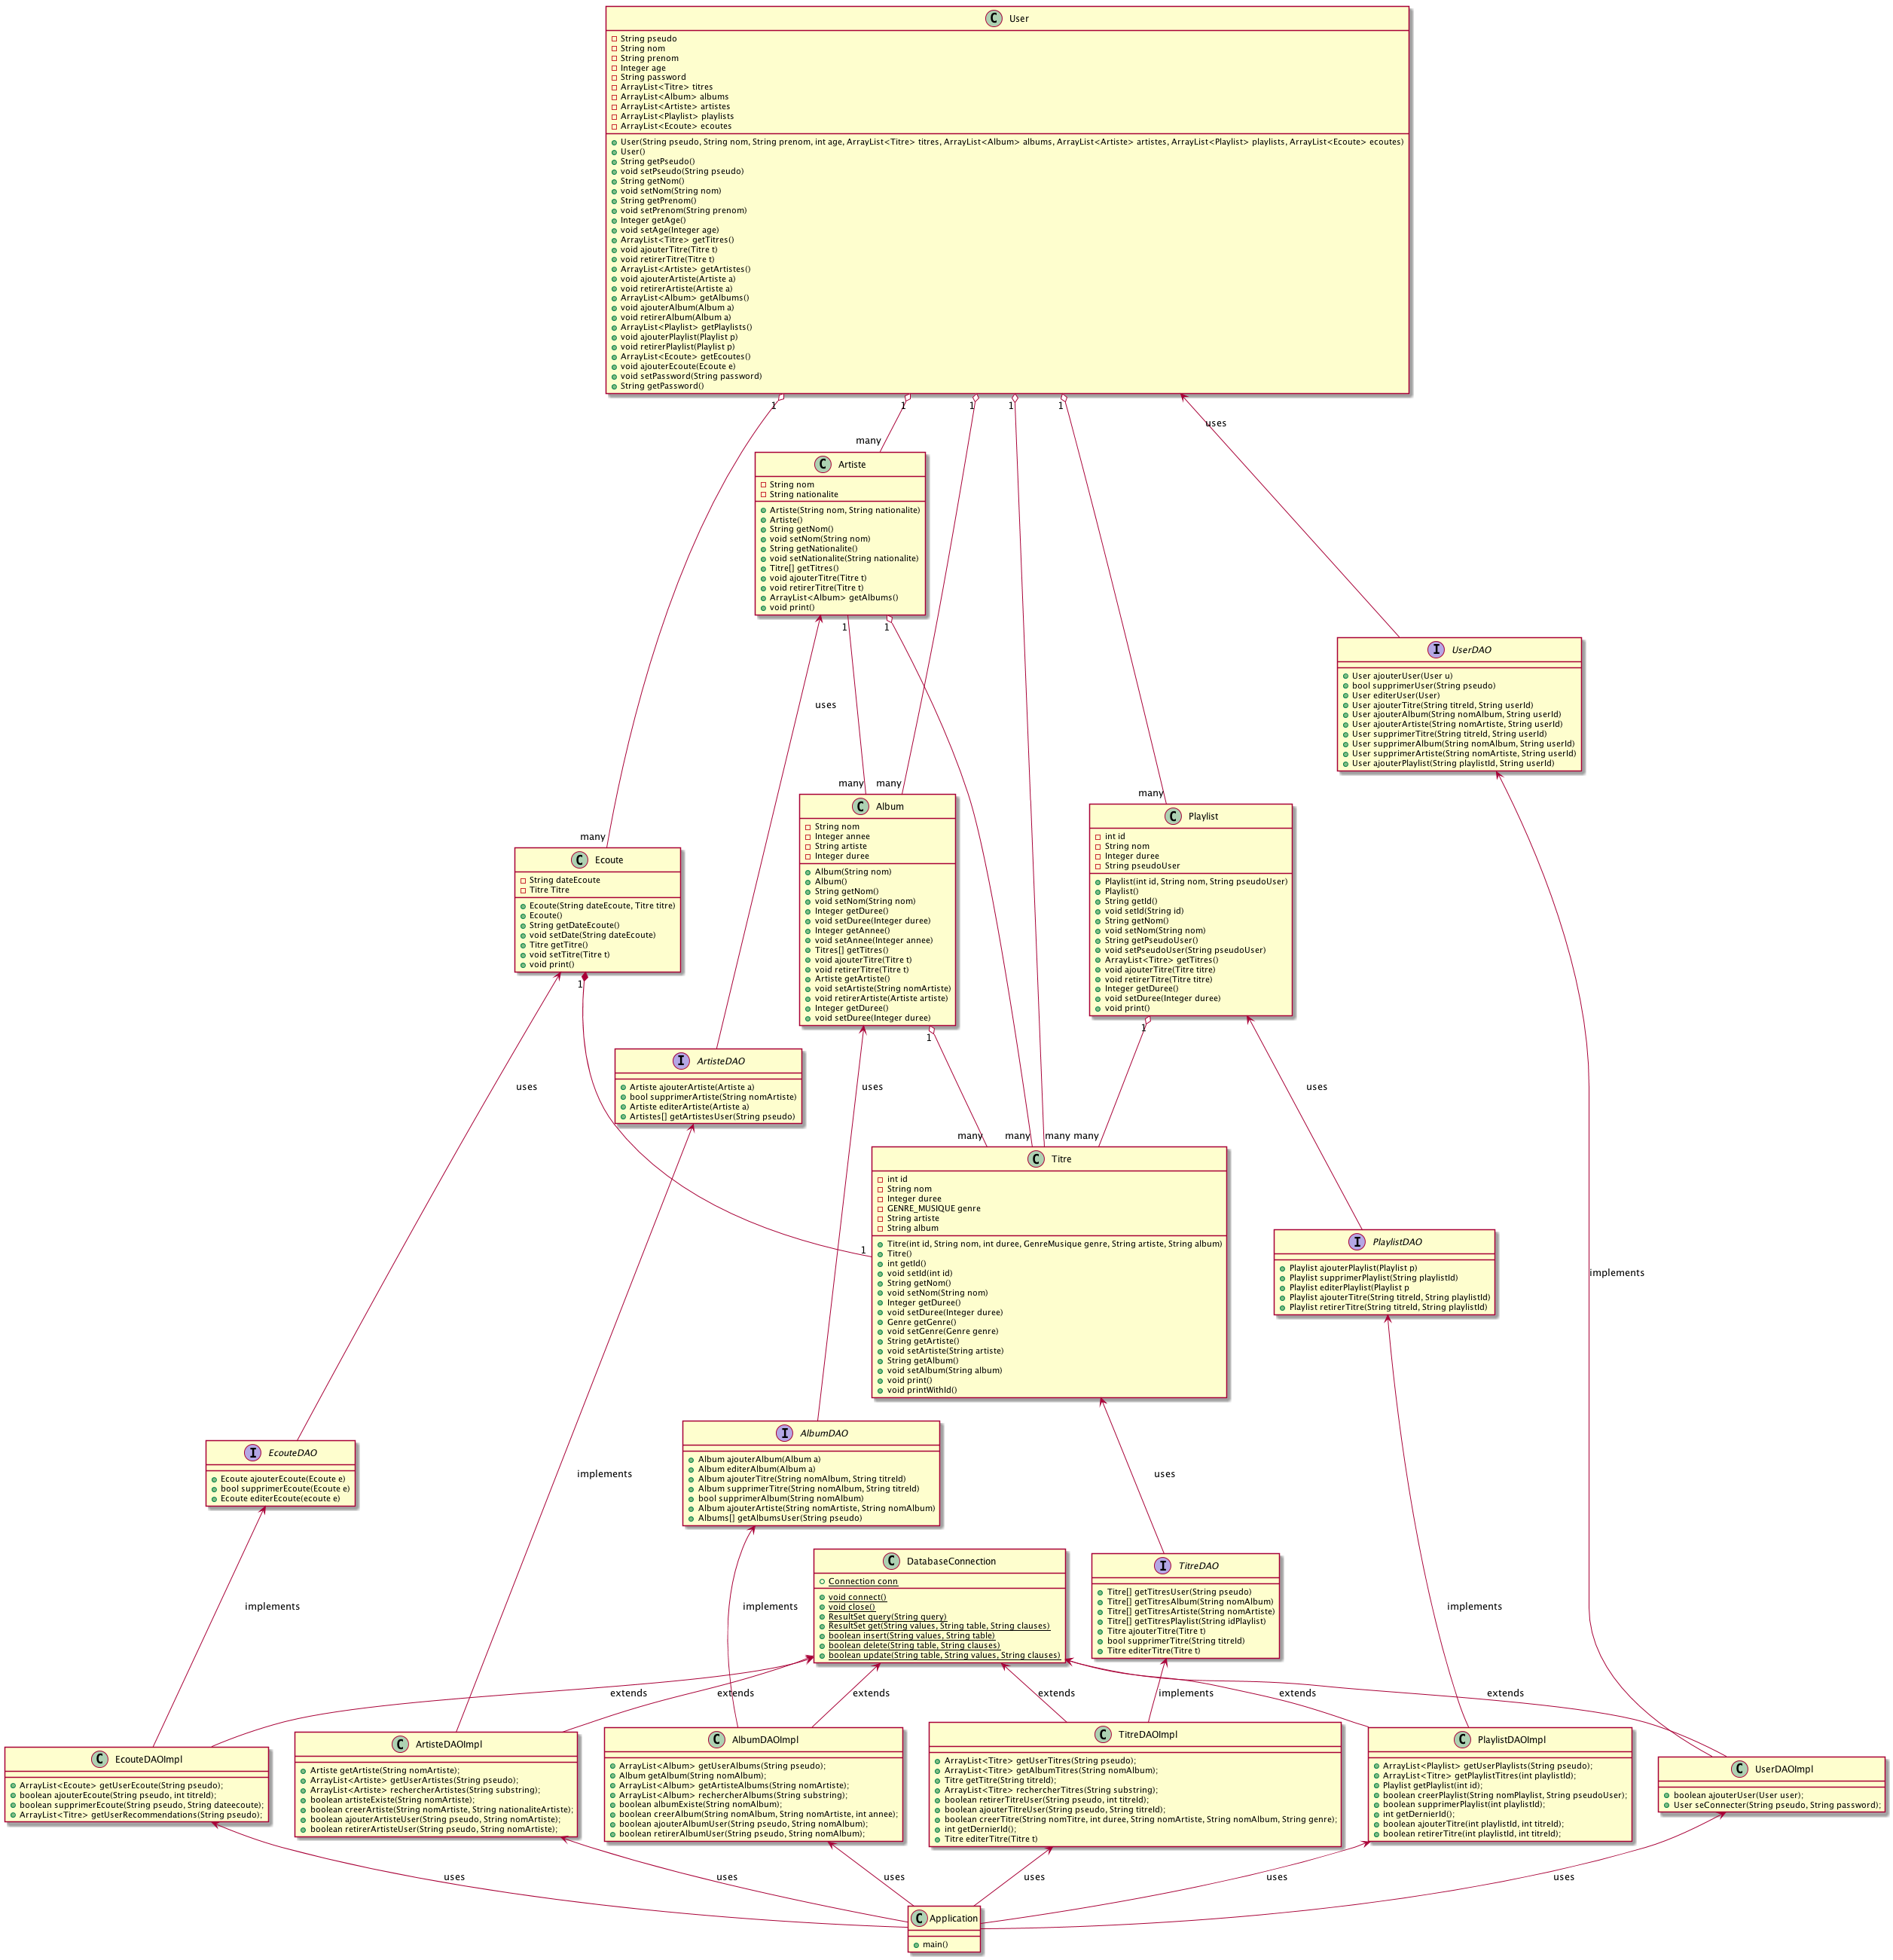
\includegraphics[scale=0.2]{class_diagram.png}
		\subsection{Package Views}
		Le package \textbf{views} contient toutes les vues de l'application. Il consiste en une agrégation de classes permettant d'afficher les vues de l'application et d'interagir avec l'utilisateur. On utilise un \textbf{singleton} \emph{MainFrameController}. Cette classe est la classe nous permettant de naviguer entre les différentes vues de l'application. Elle possède \textbf{deux attributs statiques} qui sont une instance de \emph{Scanner} nous permettant de récupérer les entrées utilisateur et une instance de \emph{User} qui est l'utilisateur connecté à l'application.
		\subsection{Package Utils}
		Le package \textbf{utils} contient l'énumération \emph{GenreMusique} correspondant à la colonne \emph{genre} dans la table \textbf{Titre}. Ce package comporte également la classe \textbf{Utils} contenant quelques fonctions utiles à la réalisation de l'application.
		\subsection{Main}
		Le \textbf{Main} a pour rôle de créer une instance de \textbf{MainFrameController} afin de lancer l'application. Le constructeur de \textbf{MainFrameController} appelle la vue de bienvenue de l'application.
	\section{Explication du fonctionnement des fonctionnalités avancées}
		\subsection{Recherche de titres, artistes, albums}
		Pour rechercher un titre, artiste, ou un album, on demande à l'utilisateur d'entrer une chaîne de caractères. On va ensuite mettre cette chaîne de caractères en minuscule et enlever les espaces de la chaîne de caractères On effectue la même opération sur la colonne \textbf{nom} de la table dans laquelle on recherche. Enfin on retourne toutes les entrées dont la chaîne de caractères recherchée est contenue dans la colonne \textbf{nom} après \textgravedbl transformation\textacutedbl. Par exemple si la musique recherchée par l'utilisateur est définie par la chaîne de caractères: \emph{giVe LifE   }, la requête sera la suivante.
		\begin{lstlisting}[language=SQL, label=rechercher,caption=Exemple de requête de recherche , breaklines, frame=single]{triggers.sql}
		SELECT * FROM TITRE WHERE strpos(lower(replace(nom, ' ', '')), 'givelife') > 0;
		\end{lstlisting}
		\subsection{Suggestion de titres}
		Pour la suggestion de titre, nous allons utiliser les écoutes saisies par l'utilisateur afin de lui proposer du contenu adapté à ces dernières. Nous allons supposer qu'un utilisateur sera susceptible d'aimer une musique si ce dernier a déjà écouté une musique de cet artiste ou encore s'il a écouté une musique dans le genre de cette musique. L'idée va donc être de récupérer les \emph{titres} en base de données que l'utilisateur n'a pas encore écoutés et dont l'artiste ou le genre est présent dans les écoutes. On va donc dans un premier temps récupérer les écoutes de l'utilisateur à partir de son \emph{pseudo}, puis extraire de ces dernières les genres et les artistes écoutés à l'aide d'une jointure intérieure avec la table titre. On obtient ainsi une matrice contenant les genres et artistes écoutés par l'utilisateur. En effectuant à nouveau une jointure intérieure avec le résultat obtenu et la table \textbf{Titre} \underline{sans les titres écoutés}, on obtient  \textbf{Titre}. L'idée est ensuite d'ordonner les résultats au hasard afin de proposer des suggestions différentes à chaque fois et de récupérer les dix premiers résultats.
		\begin{lstlisting}[language=SQL, label=rechercher,caption=Exemple de requête de suggestion , breaklines, frame=single]{triggers.sql}
		SELECT * FROM (
			SELECT * FROM TITRE WHERE id NOT IN (
				SELECT titreid as id FROM ECOUTE WHERE pseudoUser='alexis'
			)
		) as titre 	
		INNER JOIN (
			SELECT genre, nomartiste from titre INNER JOIN (
				SELECT titreId as id FROM ECOUTE WHERE pseudoUser='alexis'
			) as titresecoutes on titre.id = titresecoutes.id
		) as res on titre.genre=res.genre OR titre.nomartiste=res.nomartiste ORDER BY RANDOM() limit 10;
		\end{lstlisting}
	
		
\chapter*{Conclusion}
	Dans ce projet nous avons dans un premier temps effectué une analyse de l'objectif de l'application afin de déterminer les besoins de cette dernière. À partir de ces besoins, nous avons pu mettre en place un modèle Entité-Attribut représentant les relations, et cardinalités entre les entités et attributs de la bibliothèque musicale.Grâce à ce modèle entité-attribut, nous avons pu passer au modèle relationnel avant de concevoir puis réaliser la base de données en \textbf{PostgreSQL}. À partir de cette base de données nouvellement créée nous avons pu réaliser une application \emph{Java} de bibliothèque musicale à l'aide du driver \textbf{JDBC} nous permettant de faire le liant entre une base de données et une application. De plus cette implémentation nous a permis la découverte du pattern \textbf {DAO} permettant le passage d'un modèle relationnel à un \emph{modèle objet}. Néanmoins,il y a certaines problématiques qui n'ont pas été prises en compte dans le projet, comme le volume des données, ou encore une gestion de la concurrence intensive. 

\end{document}
